% ---------------------------------------------
% Alle Abbildungen 'images/' in Latex speichern 
%     * 'archiv/Pics-files.tex' 
%     * Bildgröße: 0.80/1 
% ju 28-Mai-2022 Pics-files.tex
% ---------------------------------------------
%
%\section{01_Generatorregel_Skizze}
%
%01_Generatorregel_Skizze (\autoref{fig:01_Generatorregel_Skizze}).% Referenz
%
\begin{figure}[!hb]% hier: !hb
    \centering
  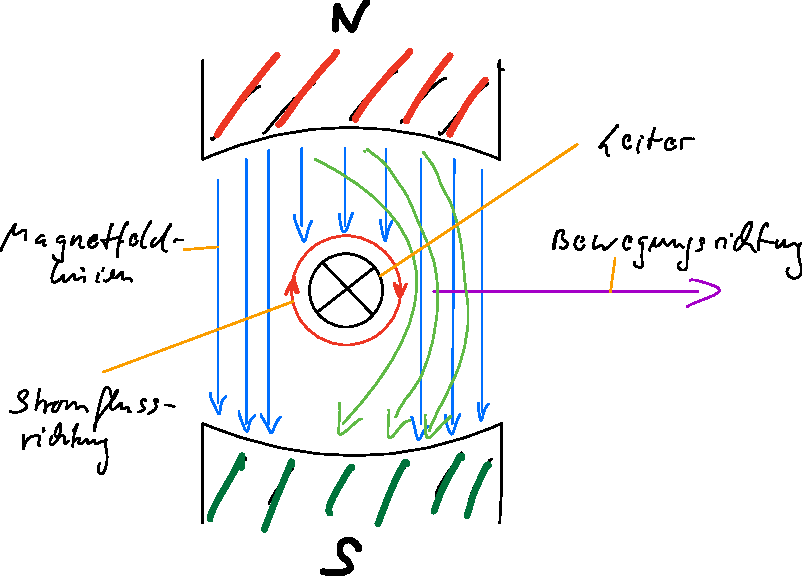
\includegraphics[width=.80\textwidth]{images/01_Generatorregel_Skizze.pdf}%
  \caption{01_Generatorregel_Skizze}%\label{fig:01_Generatorregel_Skizze}%% anpassen
\end{figure}

%\newpage
%\section{01_Schaltung_Messen_Skizze}
%
%01_Schaltung_Messen_Skizze (\autoref{fig:01_Schaltung_Messen_Skizze}).% Referenz
%
\begin{figure}[!hb]% hier: !hb
    \centering
  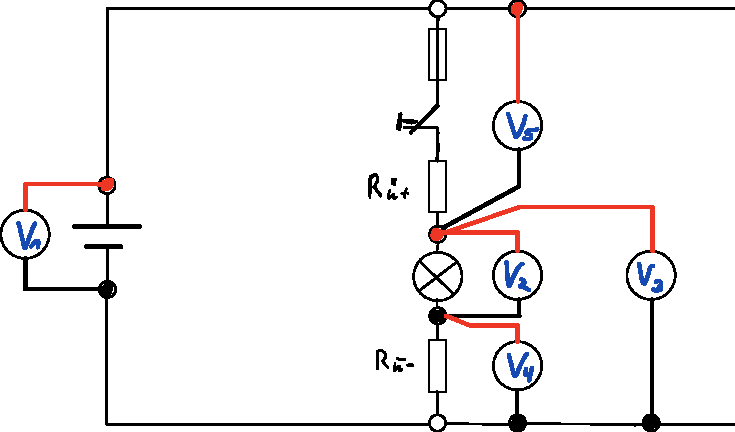
\includegraphics[width=.80\textwidth]{images/01_Schaltung_Messen_Skizze.pdf}%
  \caption{01_Schaltung_Messen_Skizze}%\label{fig:01_Schaltung_Messen_Skizze}%% anpassen
\end{figure}

%\newpage
%\section{02_Motorregel_Skizze}
%
%02_Motorregel_Skizze (\autoref{fig:02_Motorregel_Skizze}).% Referenz
%
\begin{figure}[!hb]% hier: !hb
    \centering
  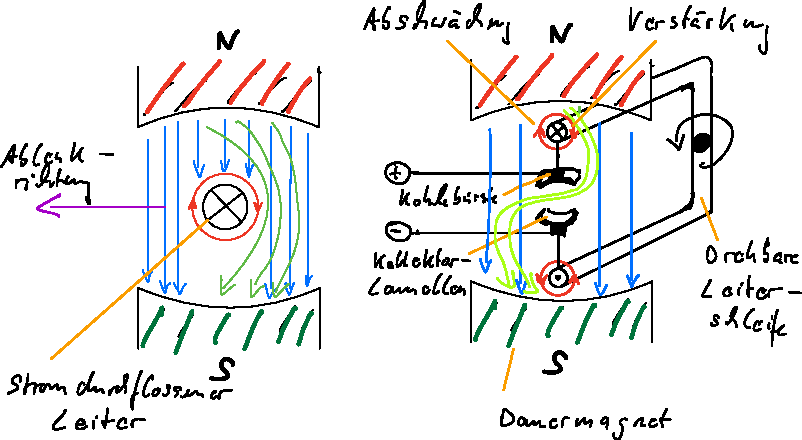
\includegraphics[width=.80\textwidth]{images/02_Motorregel_Skizze.pdf}%
  \caption{02_Motorregel_Skizze}%\label{fig:02_Motorregel_Skizze}%% anpassen
\end{figure}

%\newpage
%\section{02_Schaltung_Messen_Skizze}
%
%02_Schaltung_Messen_Skizze (\autoref{fig:02_Schaltung_Messen_Skizze}).% Referenz
%
\begin{figure}[!hb]% hier: !hb
    \centering
  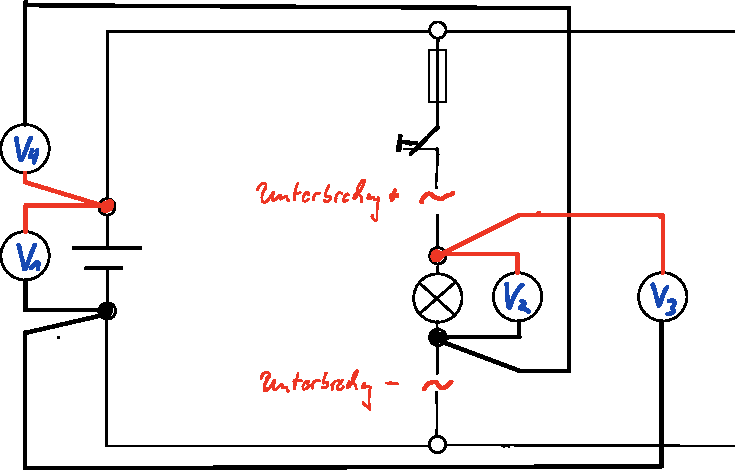
\includegraphics[width=.80\textwidth]{images/02_Schaltung_Messen_Skizze.pdf}%
  \caption{02_Schaltung_Messen_Skizze}%\label{fig:02_Schaltung_Messen_Skizze}%% anpassen
\end{figure}

%\newpage
%\section{03_Schaltung_Messen_Skizze}
%
%03_Schaltung_Messen_Skizze (\autoref{fig:03_Schaltung_Messen_Skizze}).% Referenz
%
\begin{figure}[!hb]% hier: !hb
    \centering
  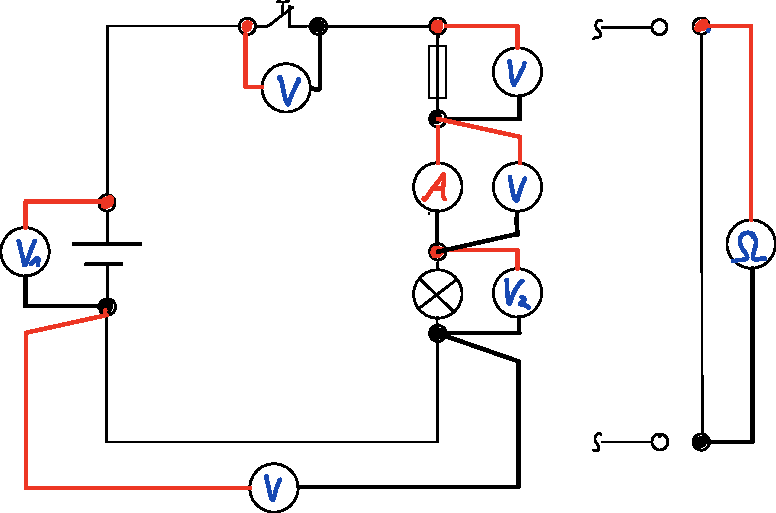
\includegraphics[width=.80\textwidth]{images/03_Schaltung_Messen_Skizze.pdf}%
  \caption{03_Schaltung_Messen_Skizze}%\label{fig:03_Schaltung_Messen_Skizze}%% anpassen
\end{figure}

%\newpage
%\section{03_StromdurchflosseneSpule_Skizze}
%
%03_StromdurchflosseneSpule_Skizze (\autoref{fig:03_StromdurchflosseneSpule_Skizze}).% Referenz
%
\begin{figure}[!hb]% hier: !hb
    \centering
  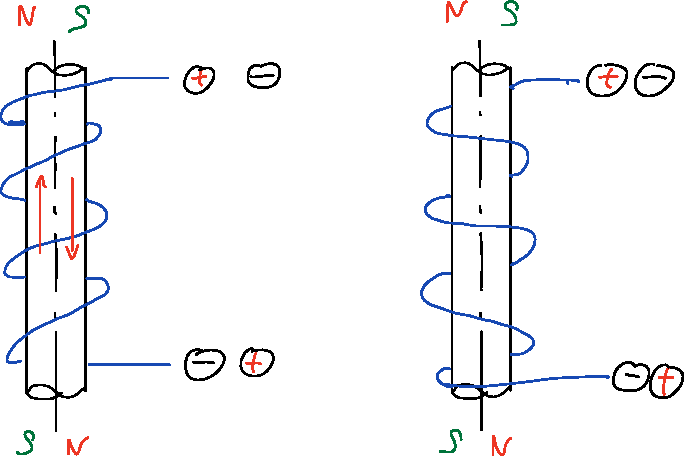
\includegraphics[width=.80\textwidth]{images/03_StromdurchflosseneSpule_Skizze.pdf}%
  \caption{03_StromdurchflosseneSpule_Skizze}%\label{fig:03_StromdurchflosseneSpule_Skizze}%% anpassen
\end{figure}

%\newpage
%\section{04_Stromdichte_Skizze}
%
%04_Stromdichte_Skizze (\autoref{fig:04_Stromdichte_Skizze}).% Referenz
%
\begin{figure}[!hb]% hier: !hb
    \centering
  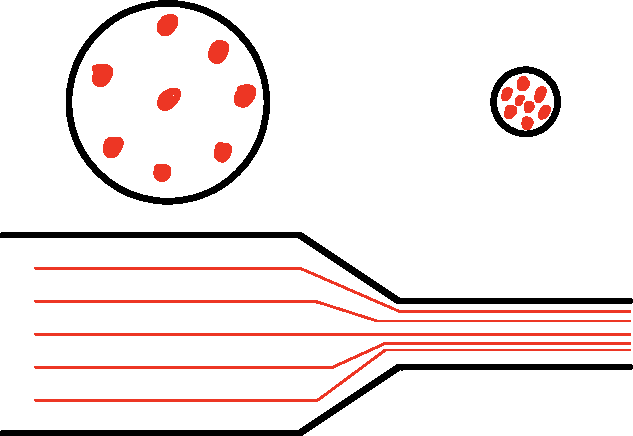
\includegraphics[width=.80\textwidth]{images/04_Stromdichte_Skizze.pdf}%
  \caption{04_Stromdichte_Skizze}%\label{fig:04_Stromdichte_Skizze}%% anpassen
\end{figure}

%\newpage
%\section{05_StromdurchflossenerLeiter_Skizze}
%
%05_StromdurchflossenerLeiter_Skizze (\autoref{fig:05_StromdurchflossenerLeiter_Skizze}).% Referenz
%
\begin{figure}[!hb]% hier: !hb
    \centering
  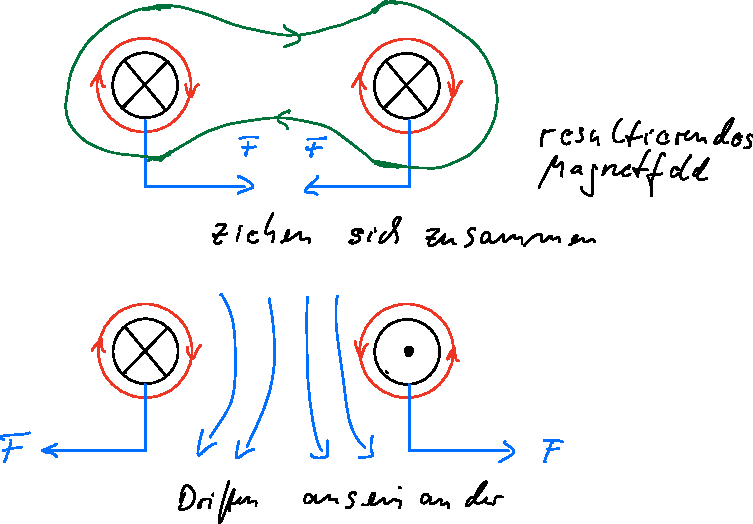
\includegraphics[width=.80\textwidth]{images/05_StromdurchflossenerLeiter_Skizze.pdf}%
  \caption{05_StromdurchflossenerLeiter_Skizze}%\label{fig:05_StromdurchflossenerLeiter_Skizze}%% anpassen
\end{figure}

%\newpage
%\section{06_Stromfluss_Messen_Skizze}
%
%06_Stromfluss_Messen_Skizze (\autoref{fig:06_Stromfluss_Messen_Skizze}).% Referenz
%
\begin{figure}[!hb]% hier: !hb
    \centering
  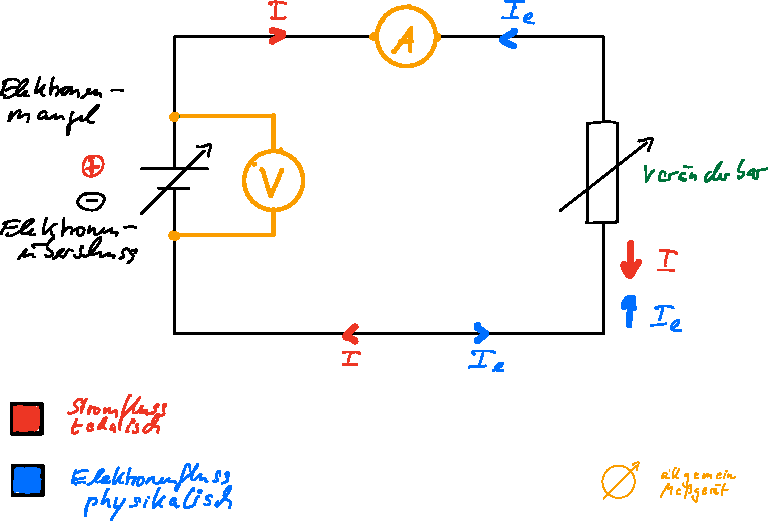
\includegraphics[width=.80\textwidth]{images/06_Stromfluss_Messen_Skizze.pdf}%
  \caption{06_Stromfluss_Messen_Skizze}%\label{fig:06_Stromfluss_Messen_Skizze}%% anpassen
\end{figure}

%\newpage
%\section{07_Reihenschaltung_Widerstaende_Skizze}
%
%07_Reihenschaltung_Widerstaende_Skizze (\autoref{fig:07_Reihenschaltung_Widerstaende_Skizze}).% Referenz
%
\begin{figure}[!hb]% hier: !hb
    \centering
  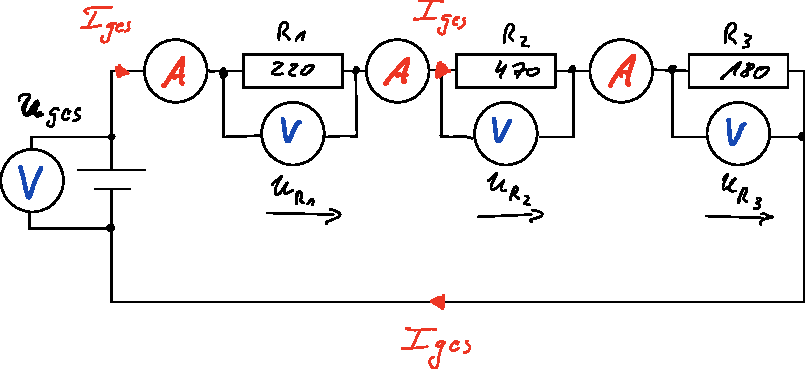
\includegraphics[width=.80\textwidth]{images/07_Reihenschaltung_Widerstaende_Skizze.pdf}%
  \caption{07_Reihenschaltung_Widerstaende_Skizze}%\label{fig:07_Reihenschaltung_Widerstaende_Skizze}%% anpassen
\end{figure}

%\newpage
%\section{08_Relais_Skizze}
%
%08_Relais_Skizze (\autoref{fig:08_Relais_Skizze}).% Referenz
%
\begin{figure}[!hb]% hier: !hb
    \centering
  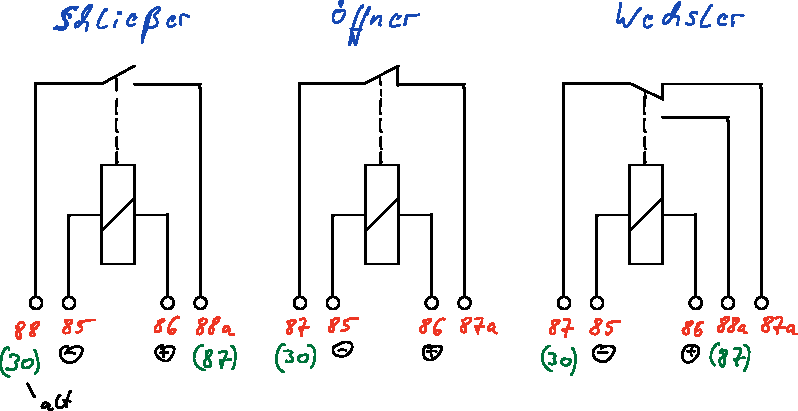
\includegraphics[width=.80\textwidth]{images/08_Relais_Skizze.pdf}%
  \caption{08_Relais_Skizze}%\label{fig:08_Relais_Skizze}%% anpassen
\end{figure}

%\newpage
%\section{09_Stroeme_einer_Relaisschaltung_Skizze}
%
%09_Stroeme_einer_Relaisschaltung_Skizze (\autoref{fig:09_Stroeme_einer_Relaisschaltung_Skizze}).% Referenz
%
\begin{figure}[!hb]% hier: !hb
    \centering
  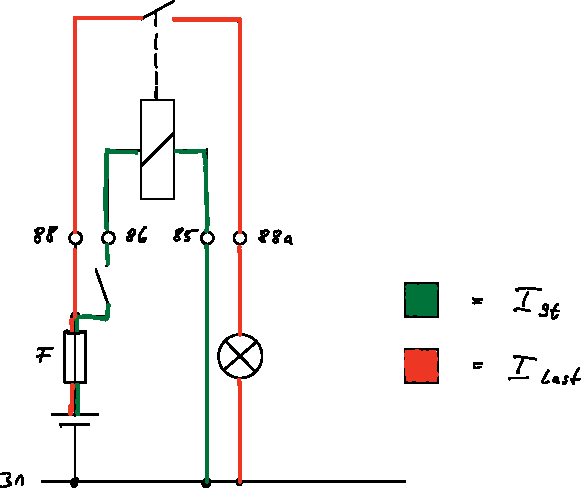
\includegraphics[width=.80\textwidth]{images/09_Stroeme_einer_Relaisschaltung_Skizze.pdf}%
  \caption{09_Stroeme_einer_Relaisschaltung_Skizze}%\label{fig:09_Stroeme_einer_Relaisschaltung_Skizze}%% anpassen
\end{figure}

%\newpage
%\section{10_Stromrelais_Skizze}
%
%10_Stromrelais_Skizze (\autoref{fig:10_Stromrelais_Skizze}).% Referenz
%
\begin{figure}[!hb]% hier: !hb
    \centering
  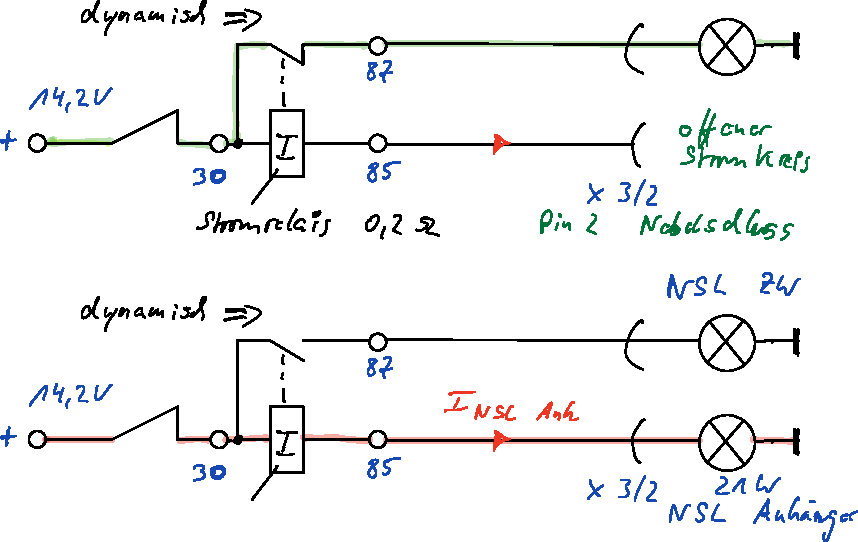
\includegraphics[width=.80\textwidth]{images/10_Stromrelais_Skizze.pdf}%
  \caption{10_Stromrelais_Skizze}%\label{fig:10_Stromrelais_Skizze}%% anpassen
\end{figure}

%\newpage
%\section{11_Schrittrelais_Skizze}
%
%11_Schrittrelais_Skizze (\autoref{fig:11_Schrittrelais_Skizze}).% Referenz
%
\begin{figure}[!hb]% hier: !hb
    \centering
  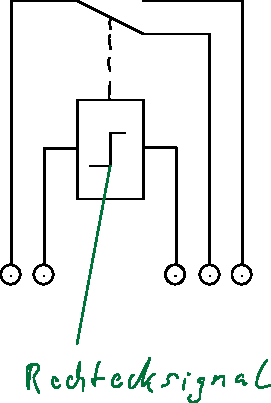
\includegraphics[width=.80\textwidth]{images/11_Schrittrelais_Skizze.pdf}%
  \caption{11_Schrittrelais_Skizze}%\label{fig:11_Schrittrelais_Skizze}%% anpassen
\end{figure}

%\newpage
%\section{12_Reedkontaktschalter_Skizze}
%
%12_Reedkontaktschalter_Skizze (\autoref{fig:12_Reedkontaktschalter_Skizze}).% Referenz
%
\begin{figure}[!hb]% hier: !hb
    \centering
  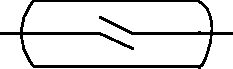
\includegraphics[width=.80\textwidth]{images/12_Reedkontaktschalter_Skizze.pdf}%
  \caption{12_Reedkontaktschalter_Skizze}%\label{fig:12_Reedkontaktschalter_Skizze}%% anpassen
\end{figure}

%\newpage
%\section{13_Spannungsverlust_Skizze}
%
%13_Spannungsverlust_Skizze (\autoref{fig:13_Spannungsverlust_Skizze}).% Referenz
%
\begin{figure}[!hb]% hier: !hb
    \centering
  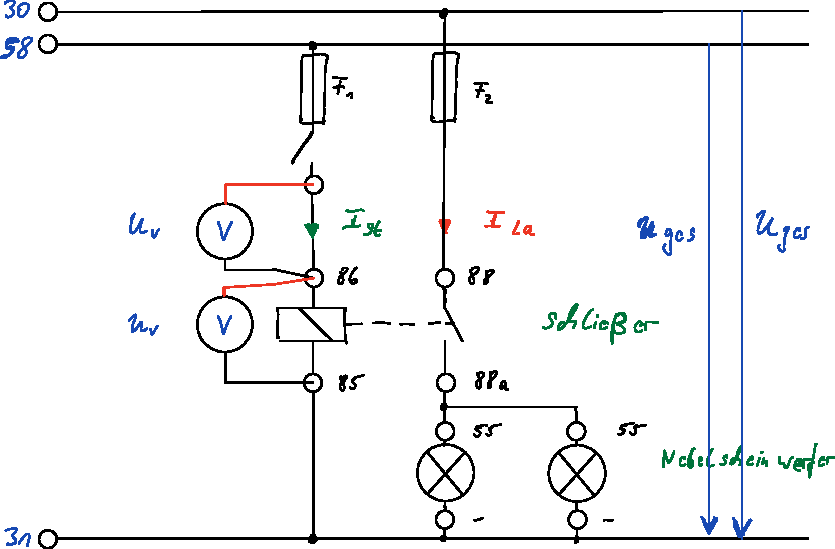
\includegraphics[width=.80\textwidth]{images/13_Spannungsverlust_Skizze.pdf}%
  \caption{13_Spannungsverlust_Skizze}%\label{fig:13_Spannungsverlust_Skizze}%% anpassen
\end{figure}

%\newpage
%\section{14_ Innenwiderstand_von_Spannungsquellen_Skizze}
%
%14_ Innenwiderstand_von_Spannungsquellen_Skizze (\autoref{fig:14_ Innenwiderstand_von_Spannungsquellen_Skizze}).% Referenz
%
\begin{figure}[!hb]% hier: !hb
    \centering
  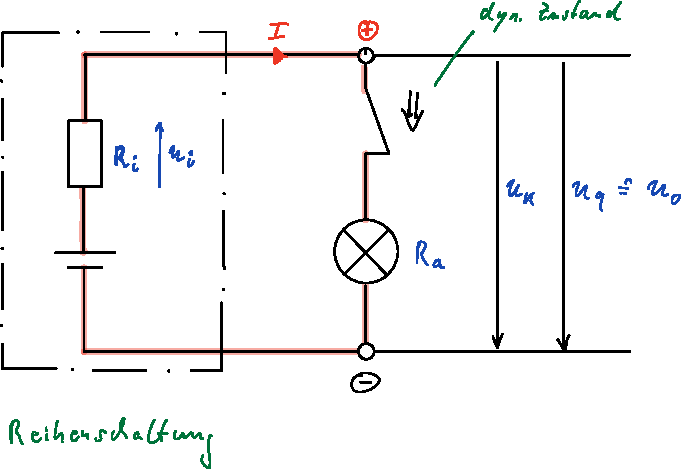
\includegraphics[width=.80\textwidth]{images/14_ Innenwiderstand_von_Spannungsquellen_Skizze.pdf}%
  \caption{14_ Innenwiderstand_von_Spannungsquellen_Skizze}%\label{fig:14_ Innenwiderstand_von_Spannungsquellen_Skizze}%% anpassen
\end{figure}

%\newpage
%\section{15_Schaltzeichen_Widerstand_Skizze}
%
%15_Schaltzeichen_Widerstand_Skizze (\autoref{fig:15_Schaltzeichen_Widerstand_Skizze}).% Referenz
%
\begin{figure}[!hb]% hier: !hb
    \centering
  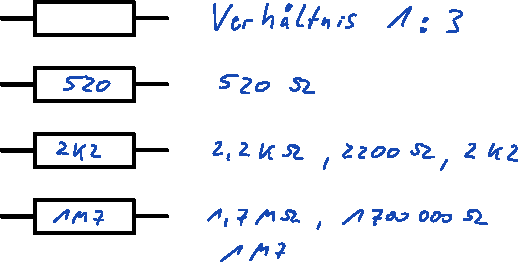
\includegraphics[width=.80\textwidth]{images/15_Schaltzeichen_Widerstand_Skizze.pdf}%
  \caption{15_Schaltzeichen_Widerstand_Skizze}%\label{fig:15_Schaltzeichen_Widerstand_Skizze}%% anpassen
\end{figure}

%\newpage
%\section{16_Widerstandsmessung_Skizze}
%
%16_Widerstandsmessung_Skizze (\autoref{fig:16_Widerstandsmessung_Skizze}).% Referenz
%
\begin{figure}[!hb]% hier: !hb
    \centering
  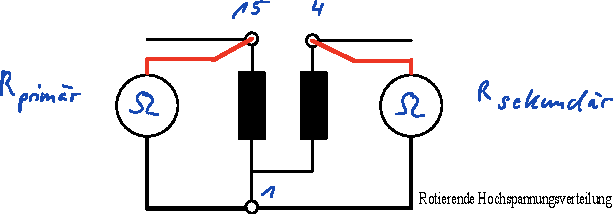
\includegraphics[width=.80\textwidth]{images/16_Widerstandsmessung_Skizze.pdf}%
  \caption{16_Widerstandsmessung_Skizze}%\label{fig:16_Widerstandsmessung_Skizze}%% anpassen
\end{figure}

%\newpage
%\section{17_Leistungsteilung_Skizze}
%
%17_Leistungsteilung_Skizze (\autoref{fig:17_Leistungsteilung_Skizze}).% Referenz
%
\begin{figure}[!hb]% hier: !hb
    \centering
  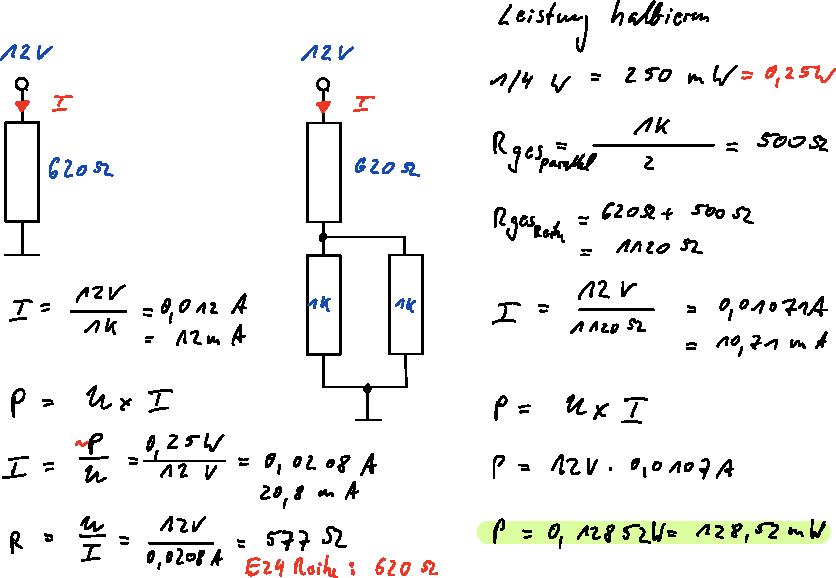
\includegraphics[width=.80\textwidth]{images/17_Leistungsteilung_Skizze.pdf}%
  \caption{17_Leistungsteilung_Skizze}%\label{fig:17_Leistungsteilung_Skizze}%% anpassen
\end{figure}

%\newpage
%\section{18_Stromflusserhoehung_Strombegrenzung_Spannungsteilung_Skizze}
%
%18_Stromflusserhoehung_Strombegrenzung_Spannungsteilung_Skizze (\autoref{fig:18_Stromflusserhoehung_Strombegrenzung_Spannungsteilung_Skizze}).% Referenz
%
\begin{figure}[!hb]% hier: !hb
    \centering
  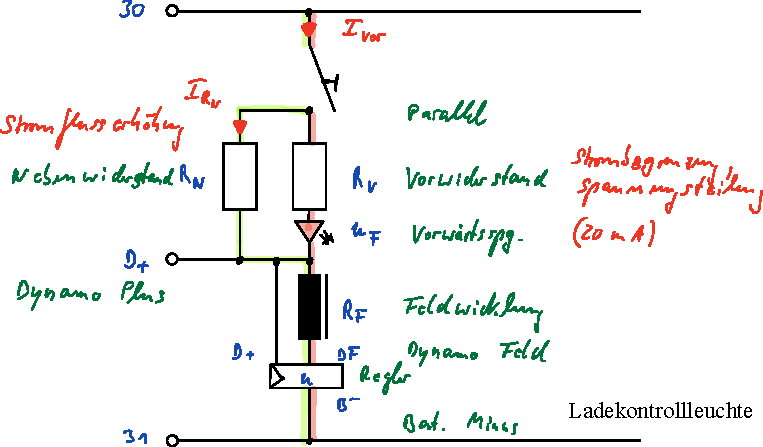
\includegraphics[width=.80\textwidth]{images/18_Stromflusserhoehung_Strombegrenzung_Spannungsteilung_Skizze.pdf}%
  \caption{18_Stromflusserhoehung_Strombegrenzung_Spannungsteilung_Skizze}%\label{fig:18_Stromflusserhoehung_Strombegrenzung_Spannungsteilung_Skizze}%% anpassen
\end{figure}

%\newpage
%\section{19_Parallelschaltung_Widerstaende_Skizze}
%
%19_Parallelschaltung_Widerstaende_Skizze (\autoref{fig:19_Parallelschaltung_Widerstaende_Skizze}).% Referenz
%
\begin{figure}[!hb]% hier: !hb
    \centering
  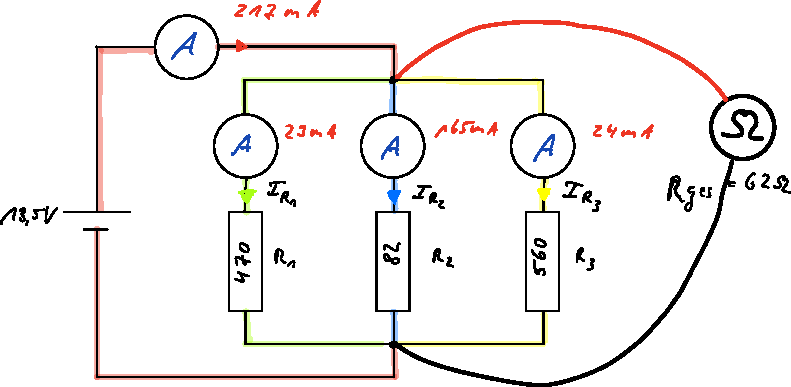
\includegraphics[width=.80\textwidth]{images/19_Parallelschaltung_Widerstaende_Skizze.pdf}%
  \caption{19_Parallelschaltung_Widerstaende_Skizze}%\label{fig:19_Parallelschaltung_Widerstaende_Skizze}%% anpassen
\end{figure}

%\newpage
%\section{20_FM_Nr5_Innenwiderstand_Aufg1_Skizze}
%
%20_FM_Nr5_Innenwiderstand_Aufg1_Skizze (\autoref{fig:20_FM_Nr5_Innenwiderstand_Aufg1_Skizze}).% Referenz
%
\begin{figure}[!hb]% hier: !hb
    \centering
  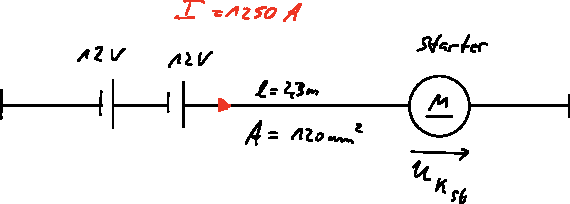
\includegraphics[width=.80\textwidth]{images/20_FM_Nr5_Innenwiderstand_Aufg1_Skizze.pdf}%
  \caption{20_FM_Nr5_Innenwiderstand_Aufg1_Skizze}%\label{fig:20_FM_Nr5_Innenwiderstand_Aufg1_Skizze}%% anpassen
\end{figure}

%\newpage
%\section{21_FM_Nr5_Innenwiderstand_Aufg2_Skizze}
%
%21_FM_Nr5_Innenwiderstand_Aufg2_Skizze (\autoref{fig:21_FM_Nr5_Innenwiderstand_Aufg2_Skizze}).% Referenz
%
\begin{figure}[!hb]% hier: !hb
    \centering
  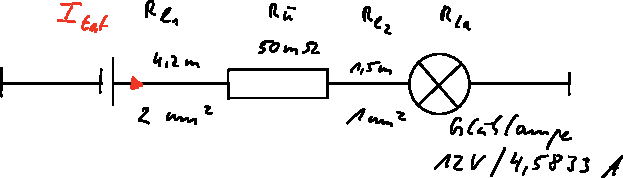
\includegraphics[width=.80\textwidth]{images/21_FM_Nr5_Innenwiderstand_Aufg2_Skizze.pdf}%
  \caption{21_FM_Nr5_Innenwiderstand_Aufg2_Skizze}%\label{fig:21_FM_Nr5_Innenwiderstand_Aufg2_Skizze}%% anpassen
\end{figure}

%\newpage
%\section{22_FM_Nr3_Reihenschaltung_Aufg3_Skizze}
%
%22_FM_Nr3_Reihenschaltung_Aufg3_Skizze (\autoref{fig:22_FM_Nr3_Reihenschaltung_Aufg3_Skizze}).% Referenz
%
\begin{figure}[!hb]% hier: !hb
    \centering
  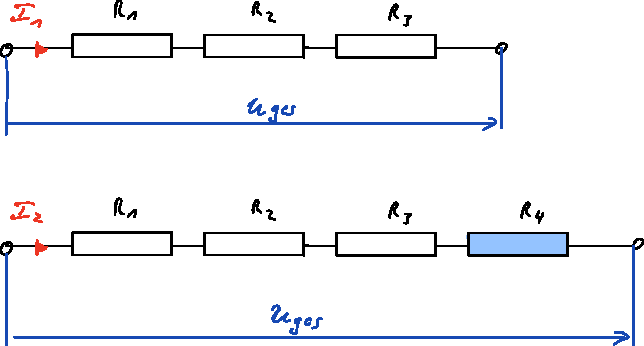
\includegraphics[width=.80\textwidth]{images/22_FM_Nr3_Reihenschaltung_Aufg3_Skizze.pdf}%
  \caption{22_FM_Nr3_Reihenschaltung_Aufg3_Skizze}%\label{fig:22_FM_Nr3_Reihenschaltung_Aufg3_Skizze}%% anpassen
\end{figure}

%\newpage
%\section{23_FM_Nr3_Reihenschaltung_Aufg4_Skizze}
%
%23_FM_Nr3_Reihenschaltung_Aufg4_Skizze (\autoref{fig:23_FM_Nr3_Reihenschaltung_Aufg4_Skizze}).% Referenz
%
\begin{figure}[!hb]% hier: !hb
    \centering
  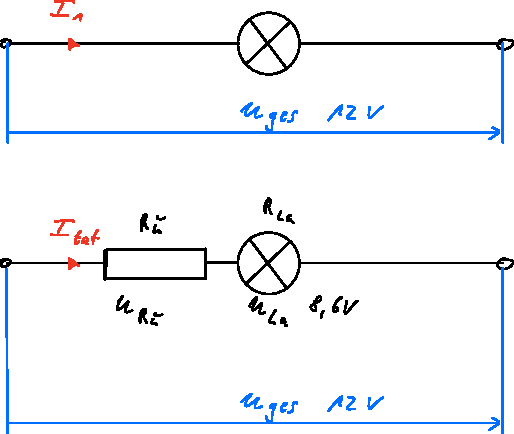
\includegraphics[width=.80\textwidth]{images/23_FM_Nr3_Reihenschaltung_Aufg4_Skizze.pdf}%
  \caption{23_FM_Nr3_Reihenschaltung_Aufg4_Skizze}%\label{fig:23_FM_Nr3_Reihenschaltung_Aufg4_Skizze}%% anpassen
\end{figure}

%\newpage
%\section{24_FM_Nr4_Reihenschaltung_Aufg4_Skizze}
%
%24_FM_Nr4_Reihenschaltung_Aufg4_Skizze (\autoref{fig:24_FM_Nr4_Reihenschaltung_Aufg4_Skizze}).% Referenz
%
\begin{figure}[!hb]% hier: !hb
    \centering
  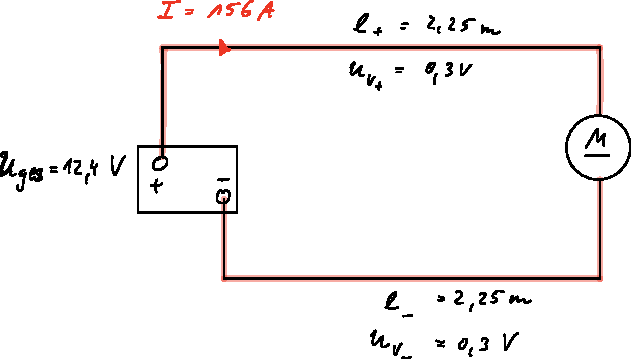
\includegraphics[width=.80\textwidth]{images/24_FM_Nr4_Reihenschaltung_Aufg4_Skizze.pdf}%
  \caption{24_FM_Nr4_Reihenschaltung_Aufg4_Skizze}%\label{fig:24_FM_Nr4_Reihenschaltung_Aufg4_Skizze}%% anpassen
\end{figure}

%\newpage
%\section{25_FM_Nr7_gemischte_Schaltung_A1}
%
%25_FM_Nr7_gemischte_Schaltung_A1 (\autoref{fig:25_FM_Nr7_gemischte_Schaltung_A1}).% Referenz
%
\begin{figure}[!hb]% hier: !hb
    \centering
  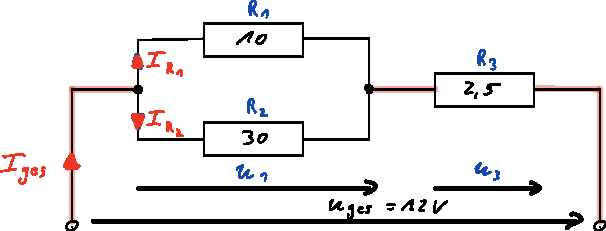
\includegraphics[width=.80\textwidth]{images/25_FM_Nr7_gemischte_Schaltung_A1.pdf}%
  \caption{25_FM_Nr7_gemischte_Schaltung_A1}%\label{fig:25_FM_Nr7_gemischte_Schaltung_A1}%% anpassen
\end{figure}

%\newpage
%\section{25_FM_Nr7_gemischte_Schaltung_A2}
%
%25_FM_Nr7_gemischte_Schaltung_A2 (\autoref{fig:25_FM_Nr7_gemischte_Schaltung_A2}).% Referenz
%
\begin{figure}[!hb]% hier: !hb
    \centering
  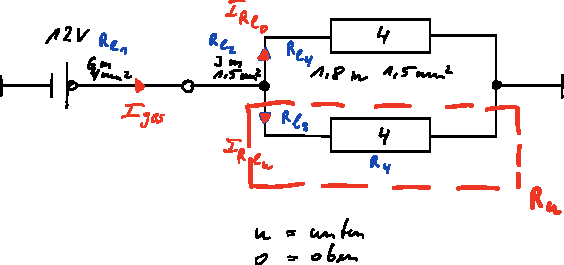
\includegraphics[width=.80\textwidth]{images/25_FM_Nr7_gemischte_Schaltung_A2.pdf}%
  \caption{25_FM_Nr7_gemischte_Schaltung_A2}%\label{fig:25_FM_Nr7_gemischte_Schaltung_A2}%% anpassen
\end{figure}

%\newpage
%\section{25_FM_Nr7_gemischte_Schaltung_A3}
%
%25_FM_Nr7_gemischte_Schaltung_A3 (\autoref{fig:25_FM_Nr7_gemischte_Schaltung_A3}).% Referenz
%
\begin{figure}[!hb]% hier: !hb
    \centering
  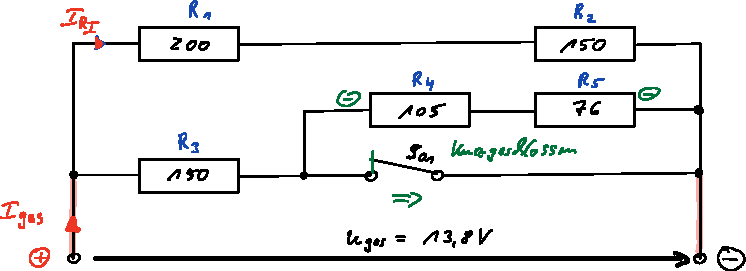
\includegraphics[width=.80\textwidth]{images/25_FM_Nr7_gemischte_Schaltung_A3.pdf}%
  \caption{25_FM_Nr7_gemischte_Schaltung_A3}%\label{fig:25_FM_Nr7_gemischte_Schaltung_A3}%% anpassen
\end{figure}

%\newpage
%\section{25_FM_Nr7_gemischte_Schaltung_A4}
%
%25_FM_Nr7_gemischte_Schaltung_A4 (\autoref{fig:25_FM_Nr7_gemischte_Schaltung_A4}).% Referenz
%
\begin{figure}[!hb]% hier: !hb
    \centering
  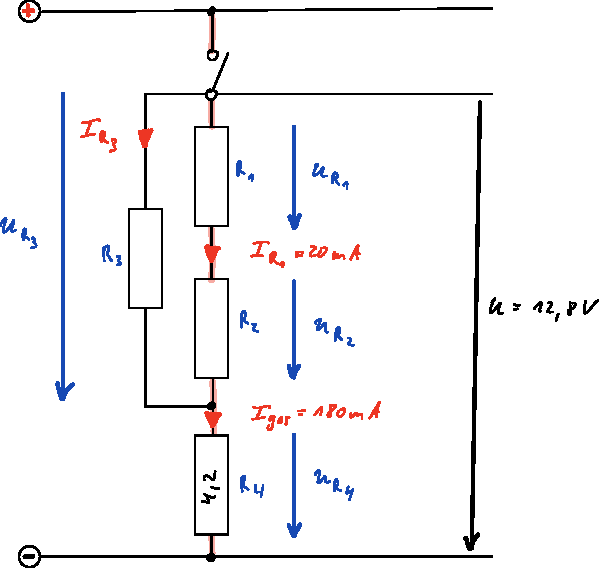
\includegraphics[width=.80\textwidth]{images/25_FM_Nr7_gemischte_Schaltung_A4.pdf}%
  \caption{25_FM_Nr7_gemischte_Schaltung_A4}%\label{fig:25_FM_Nr7_gemischte_Schaltung_A4}%% anpassen
\end{figure}

%\newpage
%\section{25_gemischte_Schaltung}
%
%25_gemischte_Schaltung (\autoref{fig:25_gemischte_Schaltung}).% Referenz
%
\begin{figure}[!hb]% hier: !hb
    \centering
  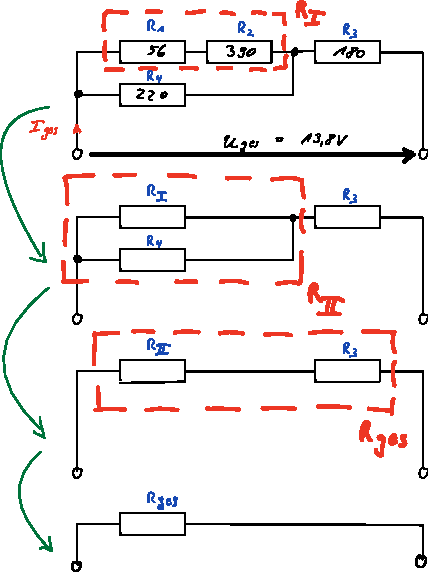
\includegraphics[width=.80\textwidth]{images/25_gemischte_Schaltung.pdf}%
  \caption{25_gemischte_Schaltung}%\label{fig:25_gemischte_Schaltung}%% anpassen
\end{figure}

%\newpage
%\section{26_FM_Leistung_Mathebuch_A3}
%
%26_FM_Leistung_Mathebuch_A3 (\autoref{fig:26_FM_Leistung_Mathebuch_A3}).% Referenz
%
\begin{figure}[!hb]% hier: !hb
    \centering
  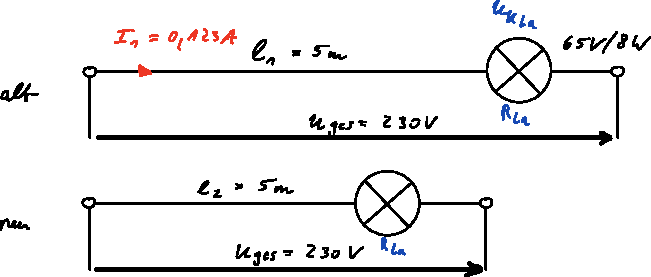
\includegraphics[width=.80\textwidth]{images/26_FM_Leistung_Mathebuch_A3.pdf}%
  \caption{26_FM_Leistung_Mathebuch_A3}%\label{fig:26_FM_Leistung_Mathebuch_A3}%% anpassen
\end{figure}

%\newpage
%\section{26_FM_Nr8_Leistung_A1}
%
%26_FM_Nr8_Leistung_A1 (\autoref{fig:26_FM_Nr8_Leistung_A1}).% Referenz
%
\begin{figure}[!hb]% hier: !hb
    \centering
  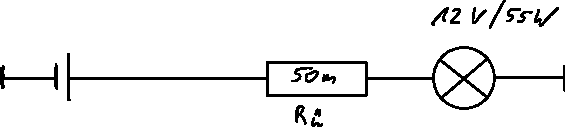
\includegraphics[width=.80\textwidth]{images/26_FM_Nr8_Leistung_A1.pdf}%
  \caption{26_FM_Nr8_Leistung_A1}%\label{fig:26_FM_Nr8_Leistung_A1}%% anpassen
\end{figure}

%\newpage
%\section{26_FM_Nr8_Leistung_A3}
%
%26_FM_Nr8_Leistung_A3 (\autoref{fig:26_FM_Nr8_Leistung_A3}).% Referenz
%
\begin{figure}[!hb]% hier: !hb
    \centering
  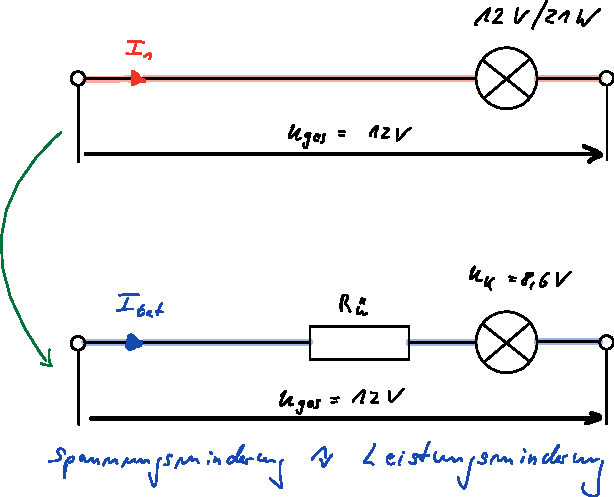
\includegraphics[width=.80\textwidth]{images/26_FM_Nr8_Leistung_A3.pdf}%
  \caption{26_FM_Nr8_Leistung_A3}%\label{fig:26_FM_Nr8_Leistung_A3}%% anpassen
\end{figure}

%\newpage
%\section{26_FM_Nr8_Leistung_A4}
%
%26_FM_Nr8_Leistung_A4 (\autoref{fig:26_FM_Nr8_Leistung_A4}).% Referenz
%
\begin{figure}[!hb]% hier: !hb
    \centering
  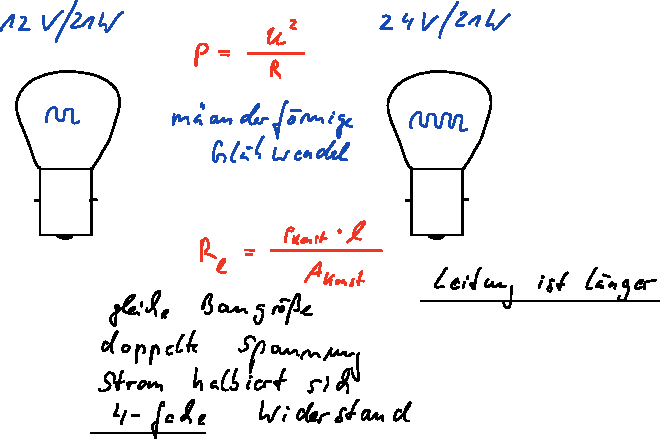
\includegraphics[width=.80\textwidth]{images/26_FM_Nr8_Leistung_A4.pdf}%
  \caption{26_FM_Nr8_Leistung_A4}%\label{fig:26_FM_Nr8_Leistung_A4}%% anpassen
\end{figure}

%\newpage
%\section{26_Leistung_Gluehlampe}
%
%26_Leistung_Gluehlampe (\autoref{fig:26_Leistung_Gluehlampe}).% Referenz
%
\begin{figure}[!hb]% hier: !hb
    \centering
  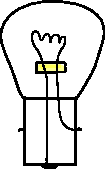
\includegraphics[width=.80\textwidth]{images/26_Leistung_Gluehlampe.pdf}%
  \caption{26_Leistung_Gluehlampe}%\label{fig:26_Leistung_Gluehlampe}%% anpassen
\end{figure}

%\newpage
%\section{27_FT_Lenkrollradius_Nachlauf}
%
%27_FT_Lenkrollradius_Nachlauf (\autoref{fig:27_FT_Lenkrollradius_Nachlauf}).% Referenz
%
\begin{figure}[!hb]% hier: !hb
    \centering
  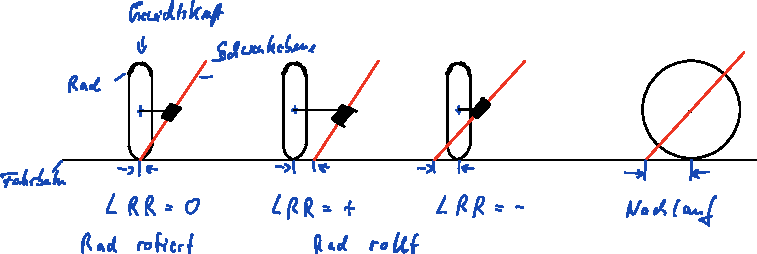
\includegraphics[width=.80\textwidth]{images/27_FT_Lenkrollradius_Nachlauf.pdf}%
  \caption{27_FT_Lenkrollradius_Nachlauf}%\label{fig:27_FT_Lenkrollradius_Nachlauf}%% anpassen
\end{figure}

%\newpage
%\section{28_FT_Brueckenschaltung}
%
%28_FT_Brueckenschaltung (\autoref{fig:28_FT_Brueckenschaltung}).% Referenz
%
\begin{figure}[!hb]% hier: !hb
    \centering
  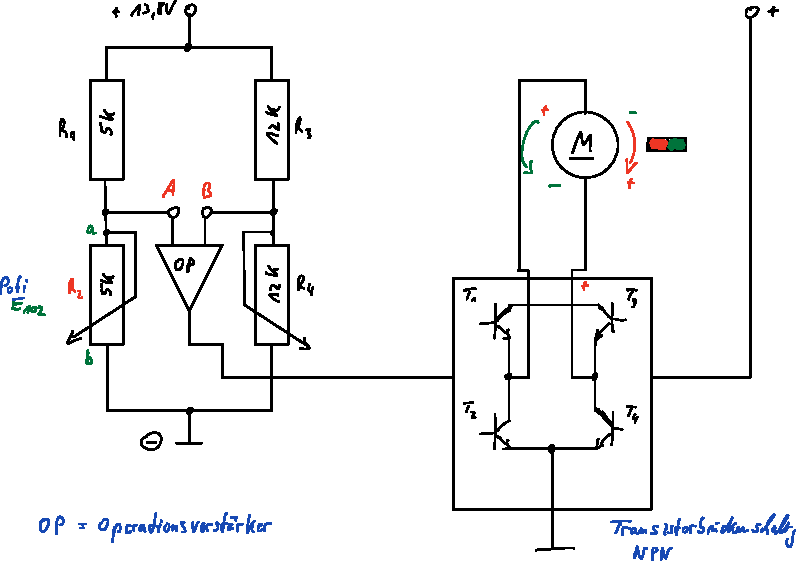
\includegraphics[width=.80\textwidth]{images/28_FT_Brueckenschaltung.pdf}%
  \caption{28_FT_Brueckenschaltung}%\label{fig:28_FT_Brueckenschaltung}%% anpassen
\end{figure}

%\newpage
%\section{28_FT_Potentialbestimmung}
%
%28_FT_Potentialbestimmung (\autoref{fig:28_FT_Potentialbestimmung}).% Referenz
%
\begin{figure}[!hb]% hier: !hb
    \centering
  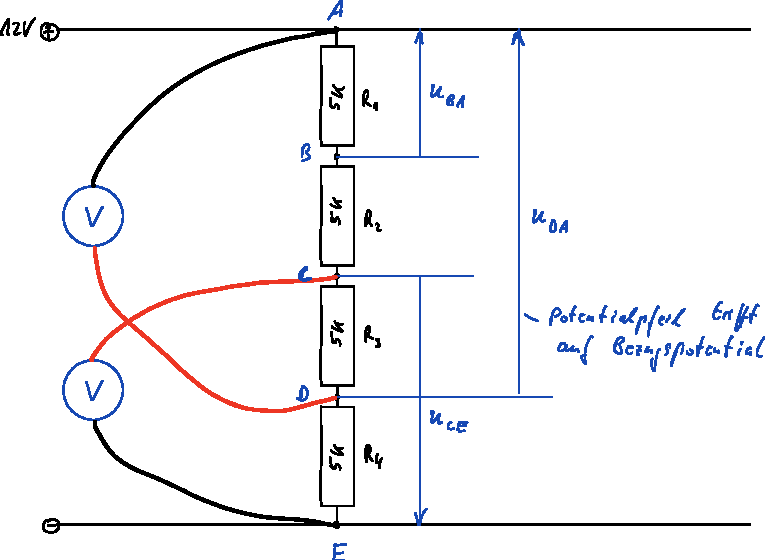
\includegraphics[width=.80\textwidth]{images/28_FT_Potentialbestimmung.pdf}%
  \caption{28_FT_Potentialbestimmung}%\label{fig:28_FT_Potentialbestimmung}%% anpassen
\end{figure}

%\newpage
%\section{28_Scheinwerferhoehenverstellung}
%
%28_Scheinwerferhoehenverstellung (\autoref{fig:28_Scheinwerferhoehenverstellung}).% Referenz
%
\begin{figure}[!hb]% hier: !hb
    \centering
  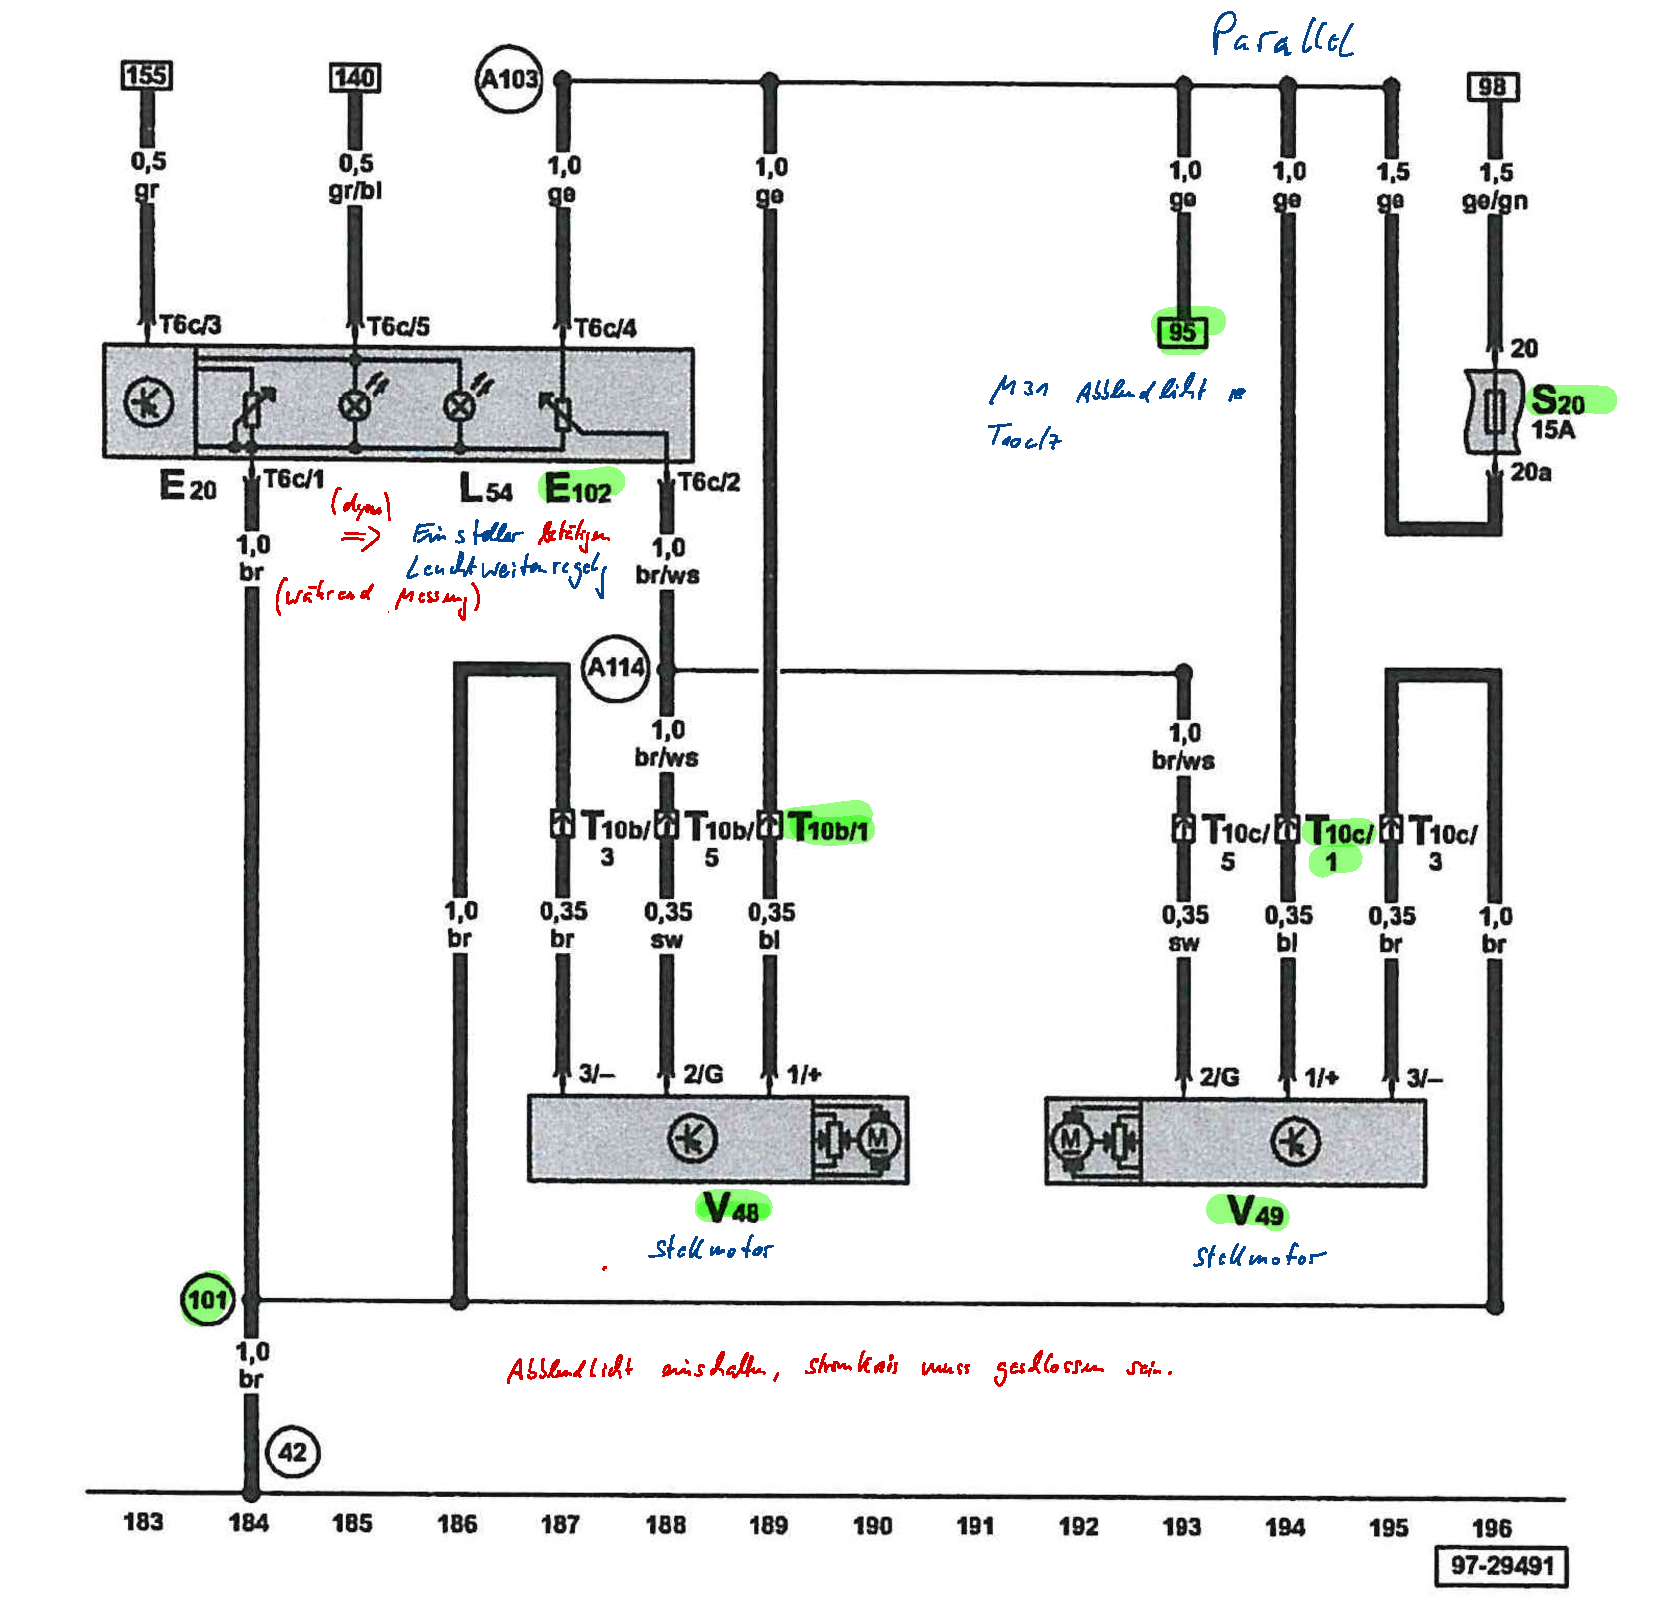
\includegraphics[width=.80\textwidth]{images/28_Scheinwerferhoehenverstellung.pdf}%
  \caption{28_Scheinwerferhoehenverstellung}%\label{fig:28_Scheinwerferhoehenverstellung}%% anpassen
\end{figure}

%\newpage
%\section{28_Scheinwerferhoehenverstellung2}
%
%28_Scheinwerferhoehenverstellung2 (\autoref{fig:28_Scheinwerferhoehenverstellung2}).% Referenz
%
\begin{figure}[!hb]% hier: !hb
    \centering
  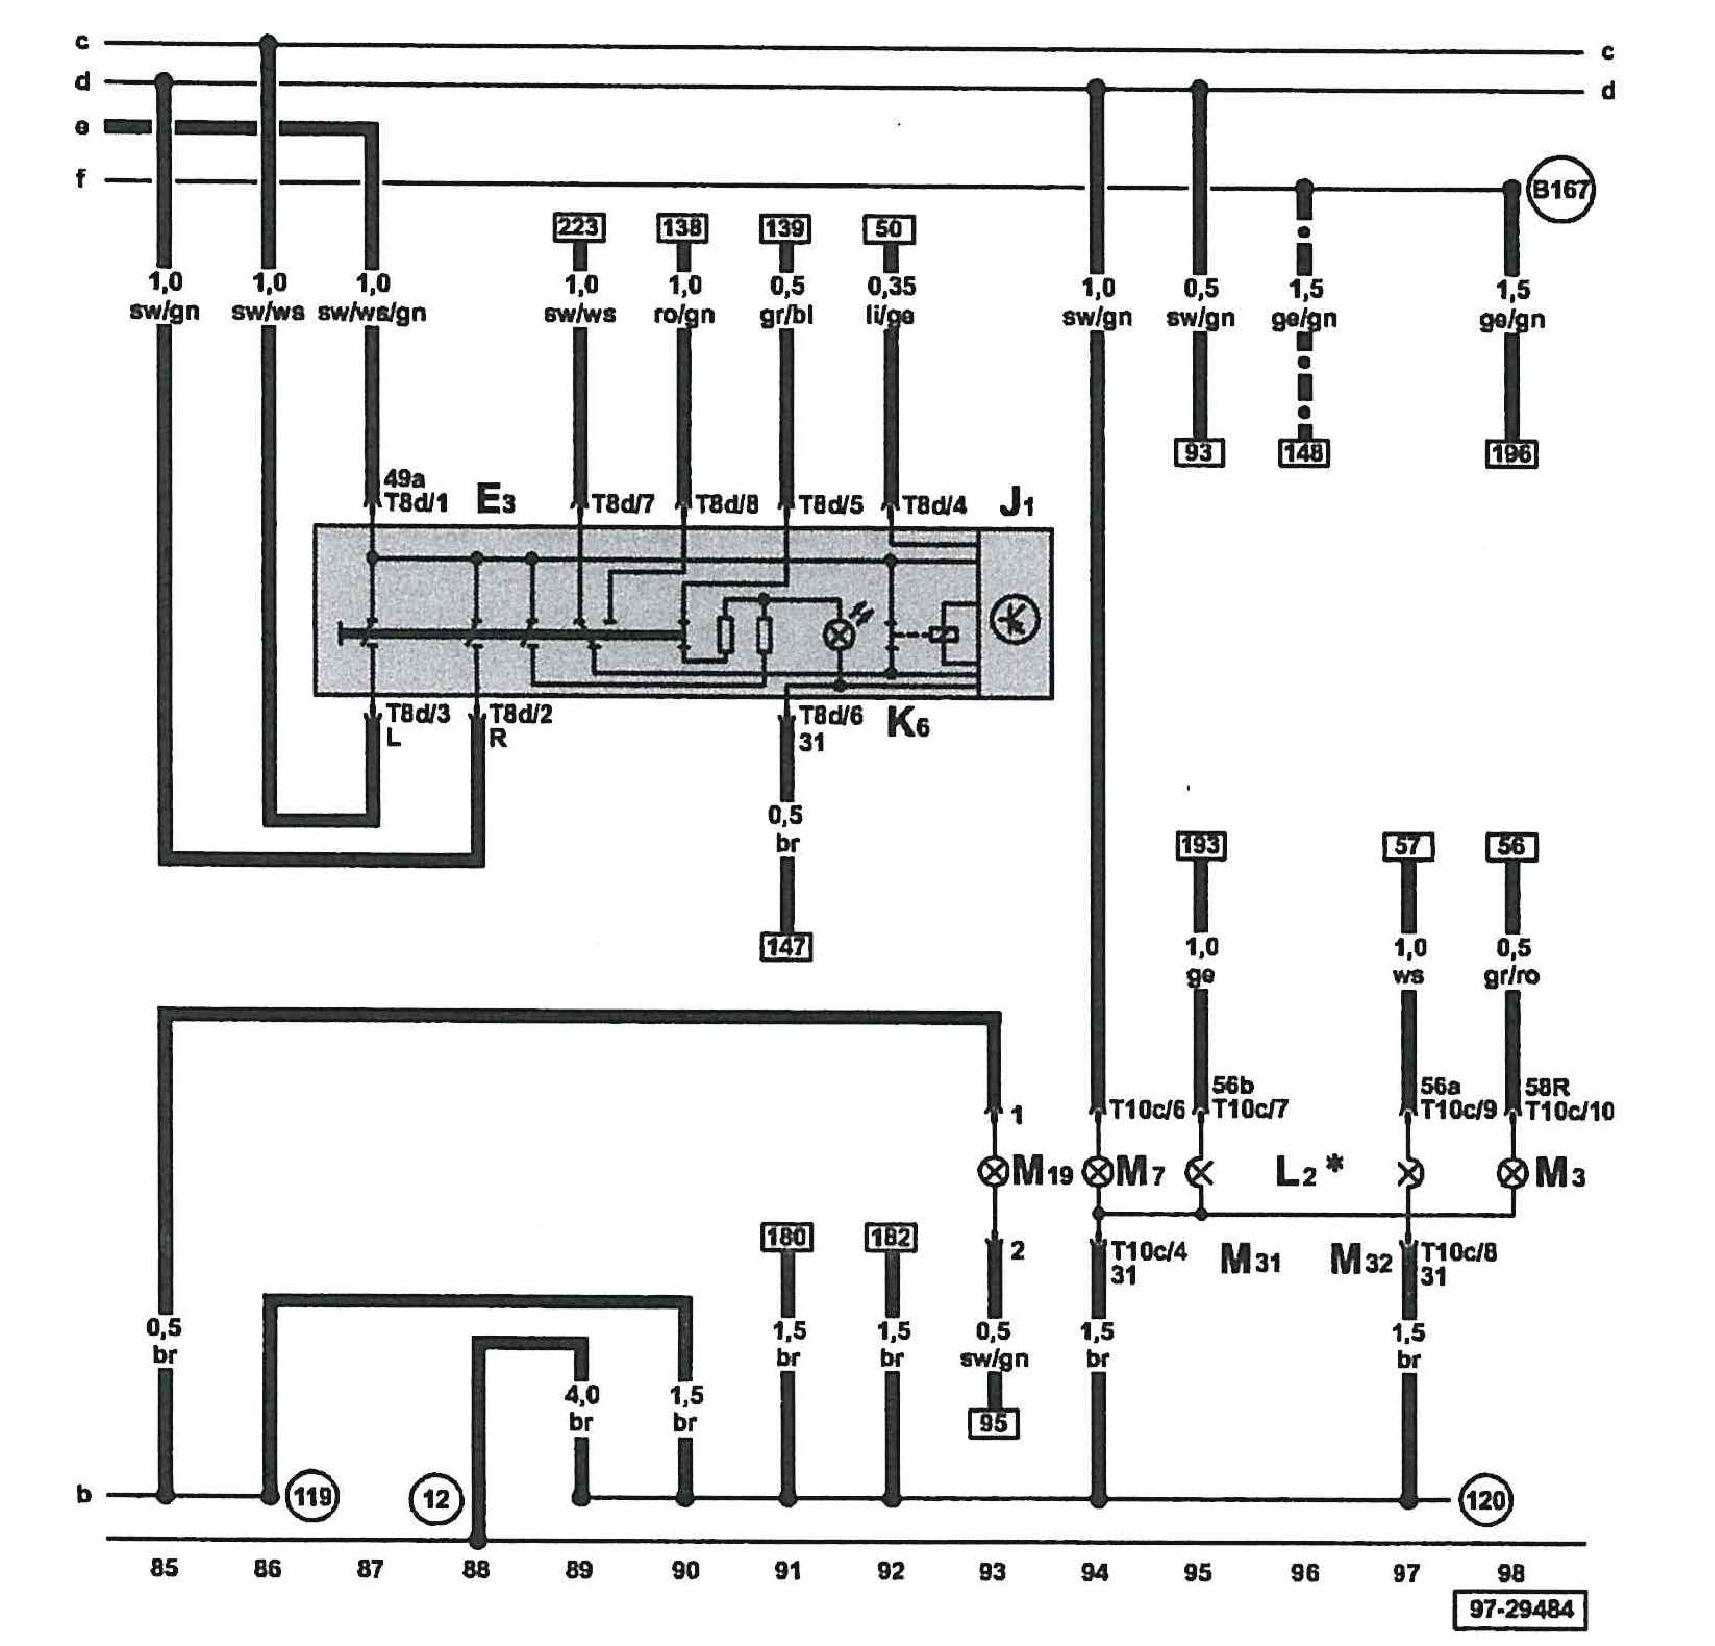
\includegraphics[width=.80\textwidth]{images/28_Scheinwerferhoehenverstellung2.pdf}%
  \caption{28_Scheinwerferhoehenverstellung2}%\label{fig:28_Scheinwerferhoehenverstellung2}%% anpassen
\end{figure}

%\newpage
%\section{29_FT_Signalanlage_Relais_6V}
%
%29_FT_Signalanlage_Relais_6V (\autoref{fig:29_FT_Signalanlage_Relais_6V}).% Referenz
%
\begin{figure}[!hb]% hier: !hb
    \centering
  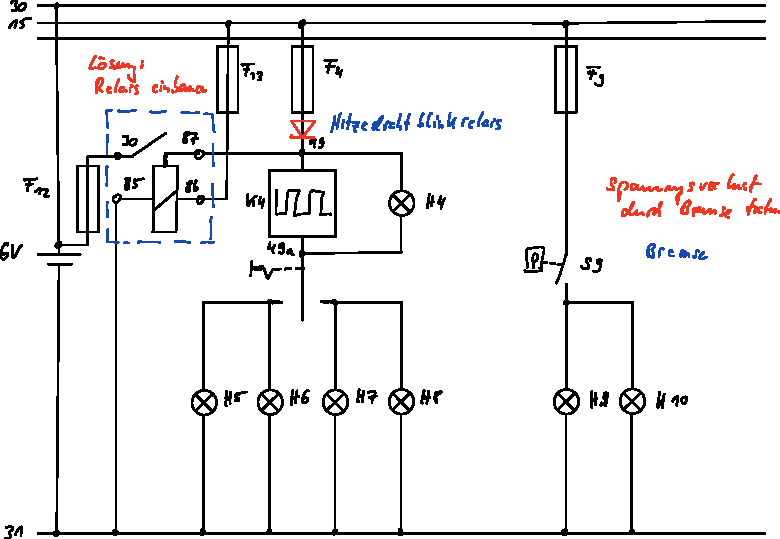
\includegraphics[width=.80\textwidth]{images/29_FT_Signalanlage_Relais_6V.pdf}%
  \caption{29_FT_Signalanlage_Relais_6V}%\label{fig:29_FT_Signalanlage_Relais_6V}%% anpassen
\end{figure}

%\newpage
%\section{29_FT_Tagfahrlicht_Relais}
%
%29_FT_Tagfahrlicht_Relais (\autoref{fig:29_FT_Tagfahrlicht_Relais}).% Referenz
%
\begin{figure}[!hb]% hier: !hb
    \centering
  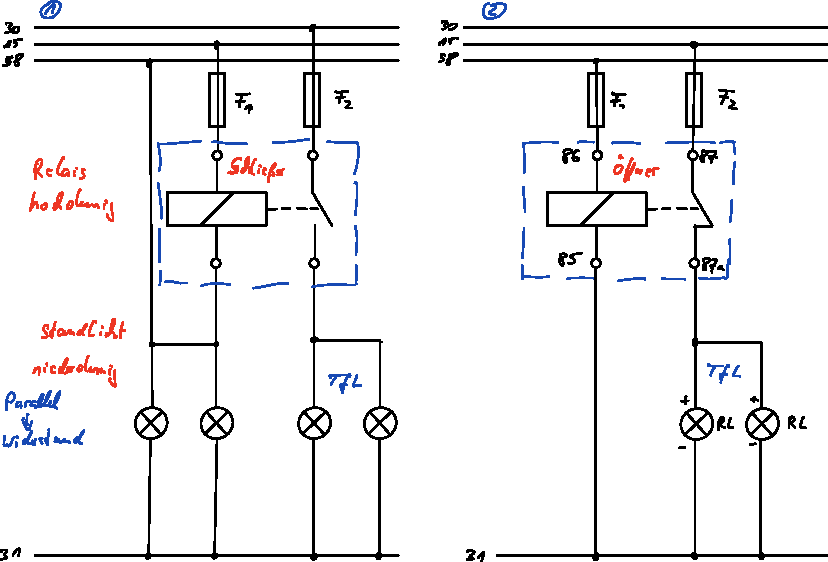
\includegraphics[width=.80\textwidth]{images/29_FT_Tagfahrlicht_Relais.pdf}%
  \caption{29_FT_Tagfahrlicht_Relais}%\label{fig:29_FT_Tagfahrlicht_Relais}%% anpassen
\end{figure}

%\newpage
%\section{29_FT_minusseitiger_Ubergangswiderstand}
%
%29_FT_minusseitiger_Ubergangswiderstand (\autoref{fig:29_FT_minusseitiger_Ubergangswiderstand}).% Referenz
%
\begin{figure}[!hb]% hier: !hb
    \centering
  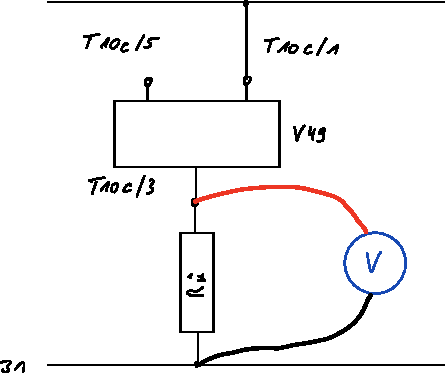
\includegraphics[width=.80\textwidth]{images/29_FT_minusseitiger_Ubergangswiderstand.pdf}%
  \caption{29_FT_minusseitiger_Ubergangswiderstand}%\label{fig:29_FT_minusseitiger_Ubergangswiderstand}%% anpassen
\end{figure}

%\newpage
%\section{30_FT_Doppelschlussmotor}
%
%30_FT_Doppelschlussmotor (\autoref{fig:30_FT_Doppelschlussmotor}).% Referenz
%
\begin{figure}[!hb]% hier: !hb
    \centering
  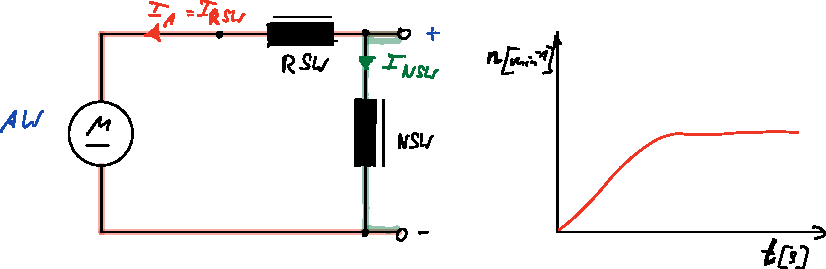
\includegraphics[width=.80\textwidth]{images/30_FT_Doppelschlussmotor.pdf}%
  \caption{30_FT_Doppelschlussmotor}%\label{fig:30_FT_Doppelschlussmotor}%% anpassen
\end{figure}

%\newpage
%\section{30_FT_Nebenschlussmotor_mit_Feldwicklung}
%
%30_FT_Nebenschlussmotor_mit_Feldwicklung (\autoref{fig:30_FT_Nebenschlussmotor_mit_Feldwicklung}).% Referenz
%
\begin{figure}[!hb]% hier: !hb
    \centering
  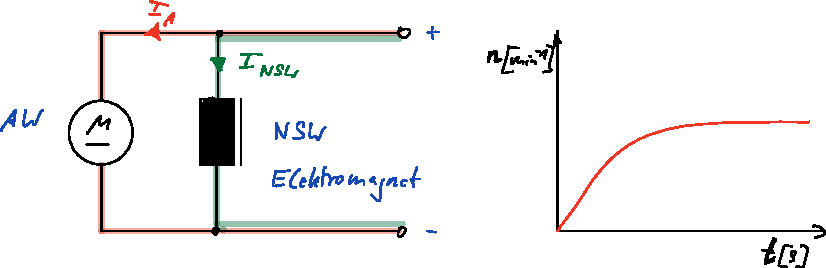
\includegraphics[width=.80\textwidth]{images/30_FT_Nebenschlussmotor_mit_Feldwicklung.pdf}%
  \caption{30_FT_Nebenschlussmotor_mit_Feldwicklung}%\label{fig:30_FT_Nebenschlussmotor_mit_Feldwicklung}%% anpassen
\end{figure}

%\newpage
%\section{30_FT_Nebenschlussmotor_mit_Permanenterregung}
%
%30_FT_Nebenschlussmotor_mit_Permanenterregung (\autoref{fig:30_FT_Nebenschlussmotor_mit_Permanenterregung}).% Referenz
%
\begin{figure}[!hb]% hier: !hb
    \centering
  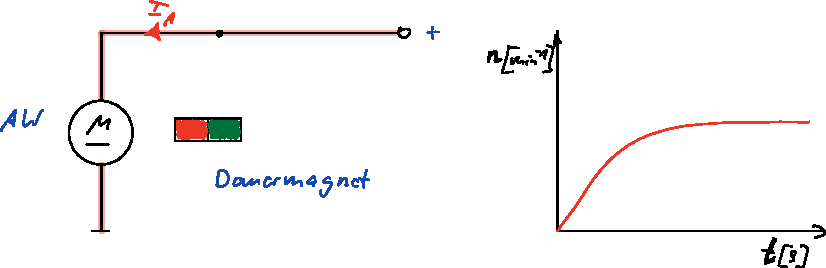
\includegraphics[width=.80\textwidth]{images/30_FT_Nebenschlussmotor_mit_Permanenterregung.pdf}%
  \caption{30_FT_Nebenschlussmotor_mit_Permanenterregung}%\label{fig:30_FT_Nebenschlussmotor_mit_Permanenterregung}%% anpassen
\end{figure}

%\newpage
%\section{30_FT_Reihenschlussmotor}
%
%30_FT_Reihenschlussmotor (\autoref{fig:30_FT_Reihenschlussmotor}).% Referenz
%
\begin{figure}[!hb]% hier: !hb
    \centering
  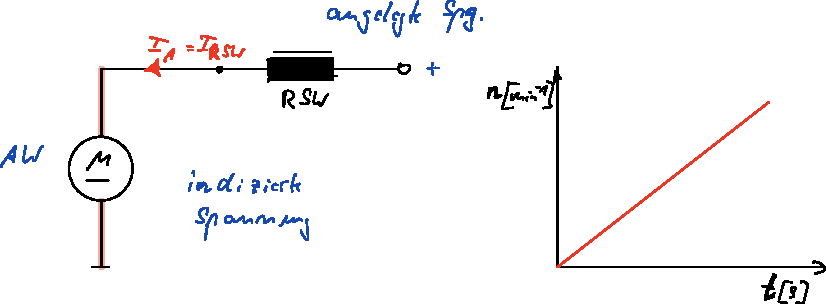
\includegraphics[width=.80\textwidth]{images/30_FT_Reihenschlussmotor.pdf}%
  \caption{30_FT_Reihenschlussmotor}%\label{fig:30_FT_Reihenschlussmotor}%% anpassen
\end{figure}

%\newpage
%\section{30_FT_Schrittmotor}
%
%30_FT_Schrittmotor (\autoref{fig:30_FT_Schrittmotor}).% Referenz
%
\begin{figure}[!hb]% hier: !hb
    \centering
  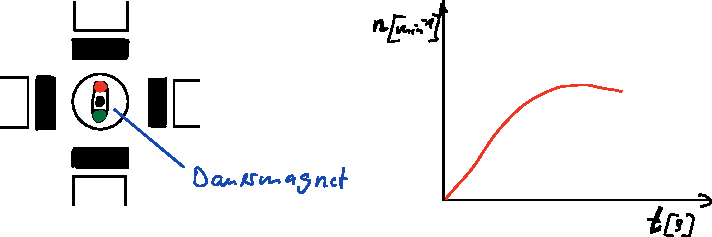
\includegraphics[width=.80\textwidth]{images/30_FT_Schrittmotor.pdf}%
  \caption{30_FT_Schrittmotor}%\label{fig:30_FT_Schrittmotor}%% anpassen
\end{figure}

%\newpage
%\section{30_FT_Wechselstrommotor}
%
%30_FT_Wechselstrommotor (\autoref{fig:30_FT_Wechselstrommotor}).% Referenz
%
\begin{figure}[!hb]% hier: !hb
    \centering
  \includegraphics[width=.80\textwidth]{images/30_FT_Wechselstrommotor.pdf}%
  \caption{30_FT_Wechselstrommotor}%\label{fig:30_FT_Wechselstrommotor}%% anpassen
\end{figure}

%\newpage
%\section{KaWa-1-Elektrotechnik-GL}
%
%KaWa-1-Elektrotechnik-GL (\autoref{fig:KaWa-1-Elektrotechnik-GL}).% Referenz
%
\begin{figure}[!hb]% hier: !hb
    \centering
  \includegraphics[width=.80\textwidth]{images/KaWa-1-Elektrotechnik-GL.pdf}%
  \caption{KaWa-1-Elektrotechnik-GL}%\label{fig:KaWa-1-Elektrotechnik-GL}%% anpassen
\end{figure}

%\newpage
%\section{Kupfer_Wuerfel_Dichte}
%
%Kupfer_Wuerfel_Dichte (\autoref{fig:Kupfer_Wuerfel_Dichte}).% Referenz
%
\begin{figure}[!hb]% hier: !hb
    \centering
  \includegraphics[width=.80\textwidth]{images/Kupfer_Wuerfel_Dichte.pdf}%
  \caption{Kupfer_Wuerfel_Dichte}%\label{fig:Kupfer_Wuerfel_Dichte}%% anpassen
\end{figure}

%\newpage
%\section{Messmethodik_Schaltkreis}
%
%Messmethodik_Schaltkreis (\autoref{fig:Messmethodik_Schaltkreis}).% Referenz
%
\begin{figure}[!hb]% hier: !hb
    \centering
  \includegraphics[width=.80\textwidth]{images/Messmethodik_Schaltkreis.pdf}%
  \caption{Messmethodik_Schaltkreis}%\label{fig:Messmethodik_Schaltkreis}%% anpassen
\end{figure}

%\newpage
